\section{Порядок выполнения лабораторной работы №1}
\begin{enumerate}
\item Выбрать вариант задания в приложении \ref{Lab1Var} в соответствии с номером в журнале. 
\item Создать в папке с номером группы на рабочем столе папку \verb#Lab1# для файлов проекта.
\item Скопировать в созданную папку \verb#Lab1#, папку CMSIS из папки \verb#LabWorkSTM32L/Materials# на рабочем столе.
\item Добавить в созданную папку с проектом папку \verb#STM32L1xx_StdPeriph_Driver# из папки \verb#LabWorkSTM32L/Materials#.
\item Добавить в созданную папку с проектом файл \verb\stm32l1xx_conf.h\ из папки \verb#LabWorkSTM32L/Materials#, добавить его в проект.
\item Добавьте в файлы \verb\stm32l1xx_gpio.c\, \verb\stm32l1xx_rcc.c\ строку:
\begin{verbatim}
#include <stm32l1xx_conf.h>
\end{verbatim}
\item Создать и настроить проект в среде разработки IAR. В качестве имени проекта указать \textit{lab1}, все файлы настроек проекта сохранить в папке \verb#Lab1#.
\item Добавить в проект IAR файлы \verb\stm32l1xx_gpio.c\, \verb\stm32l1xx_gpio.h\, \verb\stm32l1xx_rcc.c\, \verb\stm32l1xx_rcc.h\.
\item Построить блок-схему алгоритма главной программы.
\item Написать программу для микроконтроллера на языке Си.
\item Подключить отладочную плату STM32L-Discovery к компьютеру.
\item Загрузить программу в микроконтроллер и произвести ее отладку.
\item Отчет.
\end{enumerate}

\section{Пример выполнения лабораторной работы №1}
Разработать программу для микроконтроллера в среде IAR и построить блок схему алгоритма главной программы. Работа светодиодов LD3 (Green) и LD4 (Blue) задается временными диаграммами. Последовательность, приведенная на временной диаграмме, должна повторяться бесконечно.
\begin{figure}[H]
\begin{center}
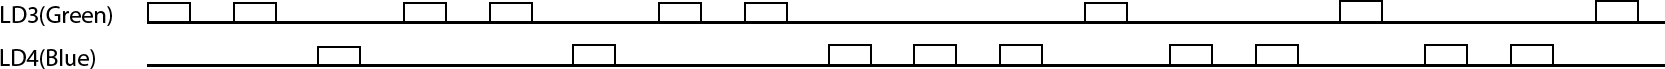
\includegraphics[scale=0.3]{Image/77.jpg} 
\end{center}
\caption{Временная диаграмма}
\end{figure}

\begin{figure}[H]
\begin{center}
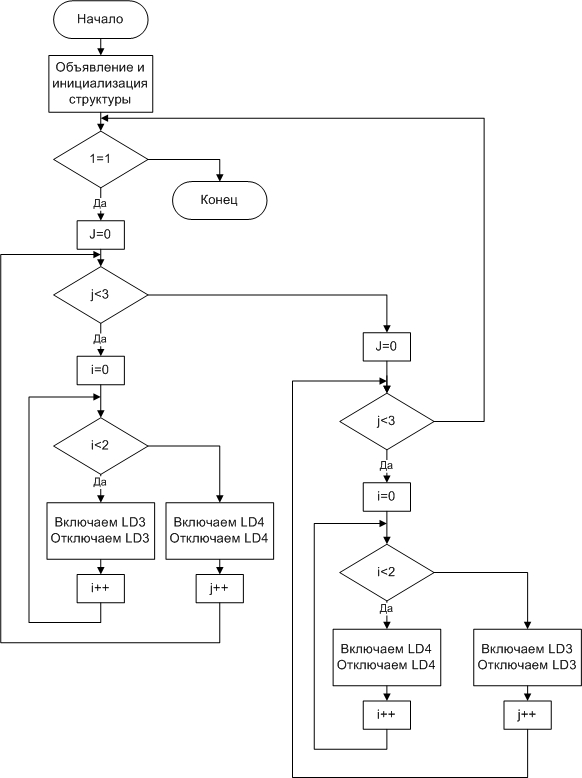
\includegraphics[scale=0.6]{Image/78.jpg} 
\end{center}
\caption{Схема алгоритма главной программы}
\end{figure}

\subsection{Пример главной программы для микроконтроллера}
\begin{verbatim}
/*################## Секция include ##################*/
#include <stm32l1xx.h>
#include <stm32l1xx_gpio.h>
#include <stm32l1xx_rcc.h>

/*################## Константы ##################*/ 
#define MAX_LOOP_NUMBER     100000 /* Количество итераций цикла 
                                      для программной задержки */

/*################## Прототипы функций ##################*/
void LAB1_Delay(uint32_t value);    
void LED3_Blink(void);              
void LED4_Blink(void);              

/*################## Опредение функций ##################*/

/*
 * Программная задержка
 * Входные данные:
 *  value - количество итерация цикла
 */
void LAB1_Delay(uint32_t value)
{
    uint32_t i;
    for (i = 0; i <= value; i++)
        ;
}

/*
 * Мигание светодиода LED3
 */
void LED3_Blink(void)
{
    GPIO_SetBits(GPIOB, GPIO_Pin_7);
    LAB1_Delay(MAX_LOOP_NUMBER);

    GPIO_ResetBits(GPIOB, GPIO_Pin_7);
    LAB1_Delay(MAX_LOOP_NUMBER);
}

/*
 * Мигание светодиода LED4
 */
void LED4_Blink(void) 
{
    GPIO_SetBits(GPIOB, GPIO_Pin_6);
    LAB1_Delay(MAX_LOOP_NUMBER);

    GPIO_ResetBits(GPIOB, GPIO_Pin_6);
    LAB1_Delay(MAX_LOOP_NUMBER);
}

/*################## Программа ##################*/
void main(void)
{
    uint32_t            i, j;
    GPIO_InitTypeDef    GPIO_InitStructure;             

    GPIO_InitStructure.GPIO_Pin   = GPIO_Pin_7 | GPIO_Pin_6 ;
    GPIO_InitStructure.GPIO_Mode  = GPIO_Mode_OUT;
    GPIO_InitStructure.GPIO_Speed = GPIO_Speed_10MHz;
    GPIO_InitStructure.GPIO_OType = GPIO_OType_PP;
    
    RCC_AHBPeriphClockCmd(RCC_AHBPeriph_GPIOB, ENABLE); /* Тактирование*/
    GPIO_Init(GPIOB, &GPIO_InitStructure);              /* Инициализация 
                                                           GPIO*/
    while(1)
    {
        j = 0;
        while(j < 3)
        {
            for (i = 0; i < 2; i++)
            {
                LED3_Blink();
            }
            LED4_Blink();
            j++;
        } /* end of while(j < 3) */

        j = 0;

        while(j < 3)
        {
            for (i = 0; i < 2; i++)
            {            
                LED4_Blink();
            }
            LED3_Blink();
            j++;
        } /* end of while(j < 3) */
    } /* end of while(1) */
} /* end of main() */
\end{verbatim}

\section{Варианты заданий к лабораторной работе №1}
\label{Lab1Var}
\begin{figure}[H]
\begin{center}
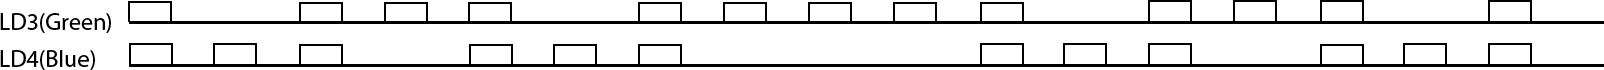
\includegraphics[scale=0.3]{Image/79.jpg} 
\end{center}
\caption{Вариант №1}
\end{figure}
\begin{figure}[H]
\begin{center}
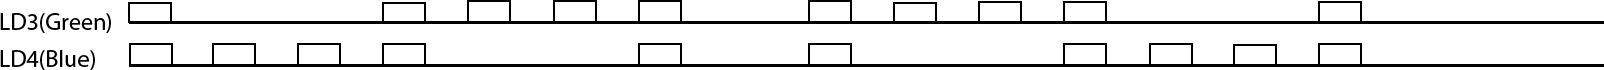
\includegraphics[scale=0.3]{Image/80.jpg} 
\end{center}
\caption{Вариант №2}
\end{figure}
\begin{figure}[H]
\begin{center}
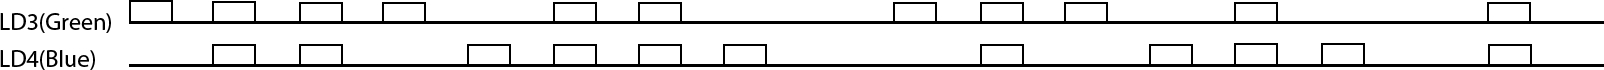
\includegraphics[scale=0.3]{Image/81.jpg} 
\end{center}
\caption{Вариант №3}
\end{figure}
\begin{figure}[H]
\begin{center}
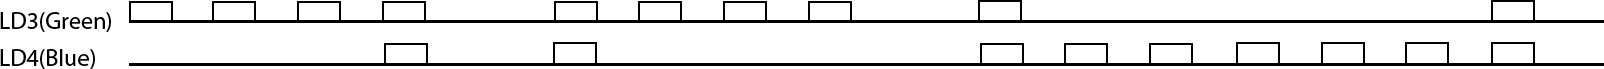
\includegraphics[scale=0.3]{Image/82.jpg} 
\end{center}
\caption{Вариант №4}
\end{figure}
\begin{figure}[H]
\begin{center}
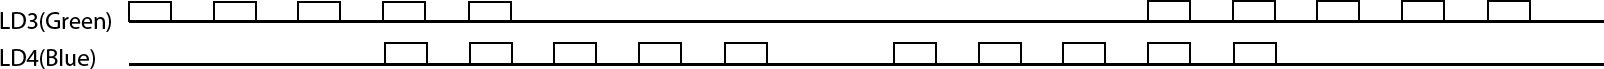
\includegraphics[scale=0.3]{Image/83.jpg} 
\end{center}
\caption{Вариант №5}
\end{figure}
\begin{figure}[H]
\begin{center}
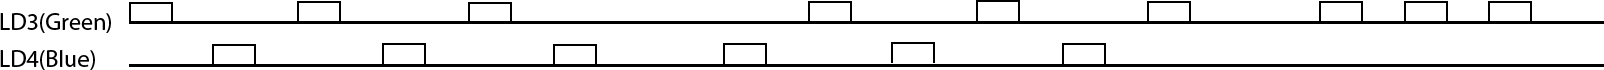
\includegraphics[scale=0.3]{Image/84.jpg} 
\end{center}
\caption{Вариант №6}
\end{figure}
\begin{figure}[H]
\begin{center}
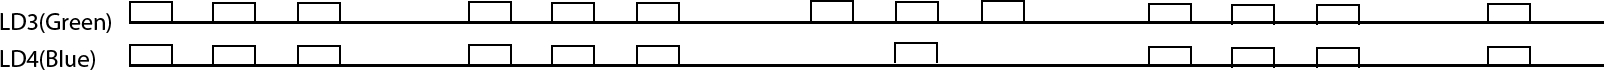
\includegraphics[scale=0.3]{Image/85.jpg} 
\end{center}
\caption{Вариант №7}
\end{figure}
\begin{figure}[H]
\begin{center}
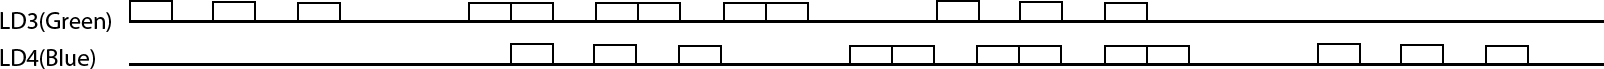
\includegraphics[scale=0.3]{Image/86.jpg} 
\end{center}
\caption{Вариант №8}
\end{figure}
\begin{figure}[H]
\begin{center}
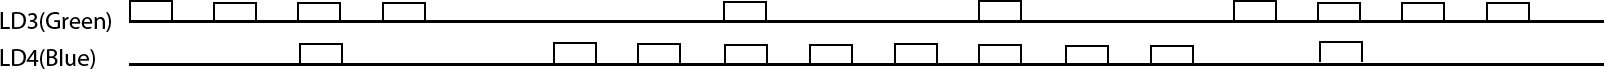
\includegraphics[scale=0.3]{Image/87.jpg} 
\end{center}
\caption{Вариант №9}
\end{figure}